Dopo aver montato il circuito in Figura \ref{fig:Circuit}, connettiamo il segnale $V_0$ all'ingresso analogico A0 della scheda Arduino Due. Utilizziamo la scheda custom contenente fotodiodo VIS/IR e diodo LED IR mostrata nella Figura \ref{fig:HRS}, utilizzando il datasheet dei componenti per definire la polarità degli stessi.
\begin{figure}[H]
    \centering
    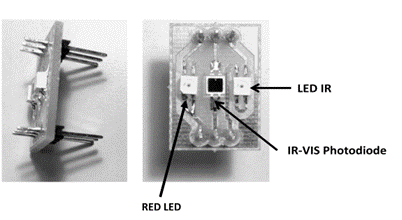
\includegraphics[width=0.5\linewidth]{Sensor.png}
    \caption{Heart Rate Sensor}
    \label{fig:HRS}
\end{figure}
Per l'analisi della frequenza cardiaca utilizziamo solamente il LED infrarosso.
\subsection{Codice acquisizione}
Scrivere un codice che permetta di acquisire il segnale in uscita al cardiofrequenzimetro, graficandolo sul display TFT allo stesso tempo. Si utilizzi per il momento il LED infrarosso per questa analisi
\begin{lstlisting}[frame=single, language=Arduino]
#include <SPI.h>
#include "Adafruit_GFX.h"
#include "Adafruit_HX8357.h"

#define sensorPin A0
#define PinIR 12
#define PinRED 11
#define TFT_CS 10
#define TFT_DC 9

Adafruit_HX8357 tft = Adafruit_HX8357(TFT_CS, TFT_DC,-1); 

const int displayWidth = 480;
const int arraySize = displayWidth;
const int graphHeight = 200;
const int sampleInterval = 20;

int acquire[arraySize];
\end{lstlisting}
\clearpage
\begin{lstlisting}[frame=single, language=Arduino]
void setup(){
    pinMode(PinIR,OUPUT);
    pinMode(PinRED,OUTPUT);
    analogReadResolution(12); // 12 bit ADC -> 4096 values

    tft.begin();
    tft.setRotation(3);
    tft.fillScreen(HX8357_BLACK);
    tft.setTextSize(3);
    tft.setCursor(30, graphHeight);
    tft.setTextColor(HX8357_WHITE);
    tft.println("Heart Rate Monitor");
}

void loop(){
    tft.setCursor(30, 240);
    tft.setTextColor(HX8357_WHITE);
    digitalWrite(PinIR,HIGH);
    tft.print("Inizio misurazione ...");    delay(1000);    
    tft.print("3"); delay(1000);    
    tft.print("2"); delay(1000);    
    tft.print("1"); delay(1000);
    tft.fillRect(0, 240, displayWidth, 80, HX8357_BLACK);
    acq();
    digitalWrite(PinIR,LOW);
    tft.setCursor(30, 240);
    tft.print("Scalamento della misurazione ...");
    plot_array_scaled(acquire);
    tft.fillRect(0, 240, displayWidth, 80, HX8357_BLACK);
}
\end{lstlisting}
\begin{lstlisting}[frame=single, language=Arduino]
void acq(){
    unsigned long currentMillis = 0;
    tft.fillRect(0, 0, displayWidth, graphHeight, HX8357_BLACK);
    for(int i = 0; i < arraySize; i++){
        acquire[i] = analogRead(sensorPin);
        currentMillis = millis();
        tft.drawPixel(i, map(array[i], 0, 4095, 0, graphHeight), HX8357_WHITE);
        while(millis() < currentMillis + sampleInterval);
    }
}
\end{lstlisting}
\subsection{Codice plotting}
Una volta acquisito l’array di valori, interrompere l’acquisizione. Scrivere una funzione che ri-scali l’array in modo di visualizzarlo sula metà superiore dello schermo, insieme ad eventuali altre scritte (v. esempio in figura); riportare sotto il corrispondente codice
\begin{lstlisting}[frame=single, language=Arduino]
void plot_array_scaled(int array[]){
    rescale();
    tft.fillRect(0, 0, displayWidth, graphHeight, HX8357_BLACK);
    for(int i = 0; i < arraySize; i++){
        tft.drawPixel(i, array[i], HX8357_WHITE);
    }
}
void rescale(){
    int max = findmax(acquire);
    int min = findmin(acquire);

    for(int i = 0; i < arraySize; i++){
        acquire[i] = map(acquire[i], min, max, 0, graphHeight);
    }
}

int findmax(int array[]){
    int max = array[0];
    for(int i = 0; i < arraySize; i++){
        if(array[i] > max)  max = array[i];
    }
    return max;
}

int findmin(int array[]){
    int min = array[0];
    for(int i = 0; i < arraySize; i++){
        if(array[i] < min)  min = array[i];
    }
    return min;
}
\end{lstlisting}